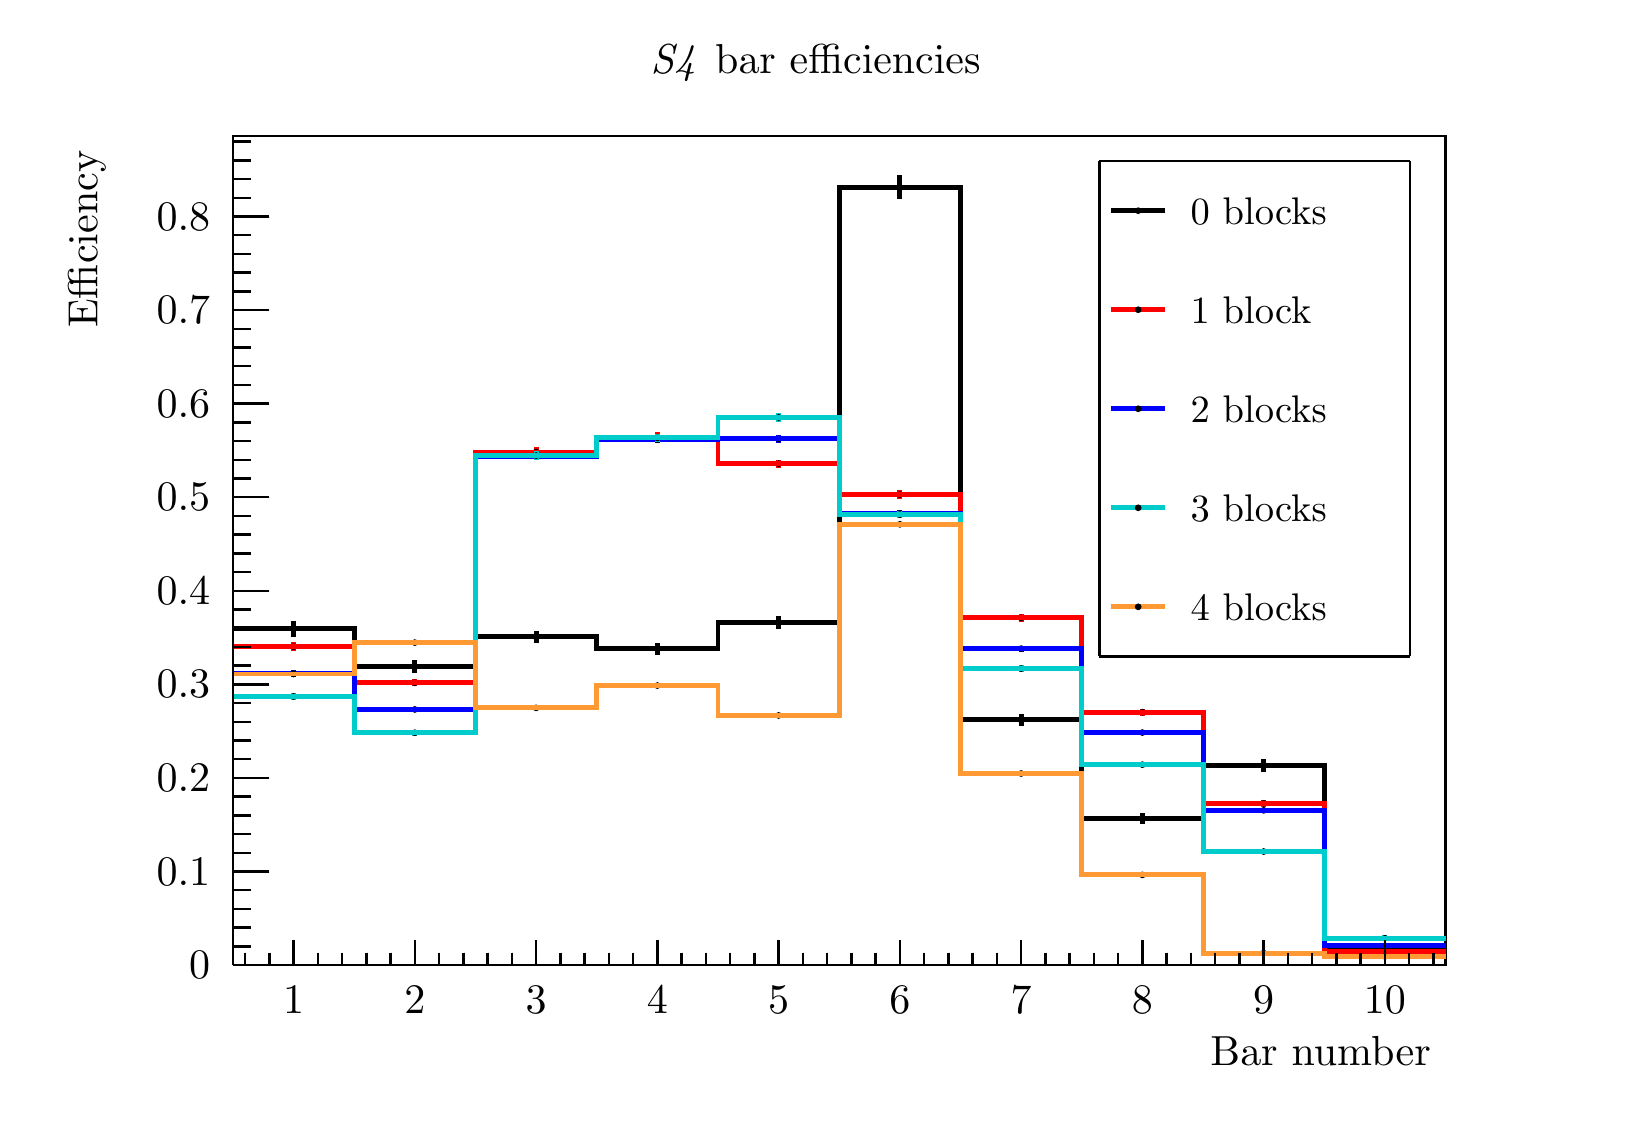
\begin{tikzpicture}
\pgfdeclareplotmark{cross} {
\pgfpathmoveto{\pgfpoint{-0.3\pgfplotmarksize}{\pgfplotmarksize}}
\pgfpathlineto{\pgfpoint{+0.3\pgfplotmarksize}{\pgfplotmarksize}}
\pgfpathlineto{\pgfpoint{+0.3\pgfplotmarksize}{0.3\pgfplotmarksize}}
\pgfpathlineto{\pgfpoint{+1\pgfplotmarksize}{0.3\pgfplotmarksize}}
\pgfpathlineto{\pgfpoint{+1\pgfplotmarksize}{-0.3\pgfplotmarksize}}
\pgfpathlineto{\pgfpoint{+0.3\pgfplotmarksize}{-0.3\pgfplotmarksize}}
\pgfpathlineto{\pgfpoint{+0.3\pgfplotmarksize}{-1.\pgfplotmarksize}}
\pgfpathlineto{\pgfpoint{-0.3\pgfplotmarksize}{-1.\pgfplotmarksize}}
\pgfpathlineto{\pgfpoint{-0.3\pgfplotmarksize}{-0.3\pgfplotmarksize}}
\pgfpathlineto{\pgfpoint{-1.\pgfplotmarksize}{-0.3\pgfplotmarksize}}
\pgfpathlineto{\pgfpoint{-1.\pgfplotmarksize}{0.3\pgfplotmarksize}}
\pgfpathlineto{\pgfpoint{-0.3\pgfplotmarksize}{0.3\pgfplotmarksize}}
\pgfpathclose
\pgfusepathqstroke
}
\pgfdeclareplotmark{cross*} {
\pgfpathmoveto{\pgfpoint{-0.3\pgfplotmarksize}{\pgfplotmarksize}}
\pgfpathlineto{\pgfpoint{+0.3\pgfplotmarksize}{\pgfplotmarksize}}
\pgfpathlineto{\pgfpoint{+0.3\pgfplotmarksize}{0.3\pgfplotmarksize}}
\pgfpathlineto{\pgfpoint{+1\pgfplotmarksize}{0.3\pgfplotmarksize}}
\pgfpathlineto{\pgfpoint{+1\pgfplotmarksize}{-0.3\pgfplotmarksize}}
\pgfpathlineto{\pgfpoint{+0.3\pgfplotmarksize}{-0.3\pgfplotmarksize}}
\pgfpathlineto{\pgfpoint{+0.3\pgfplotmarksize}{-1.\pgfplotmarksize}}
\pgfpathlineto{\pgfpoint{-0.3\pgfplotmarksize}{-1.\pgfplotmarksize}}
\pgfpathlineto{\pgfpoint{-0.3\pgfplotmarksize}{-0.3\pgfplotmarksize}}
\pgfpathlineto{\pgfpoint{-1.\pgfplotmarksize}{-0.3\pgfplotmarksize}}
\pgfpathlineto{\pgfpoint{-1.\pgfplotmarksize}{0.3\pgfplotmarksize}}
\pgfpathlineto{\pgfpoint{-0.3\pgfplotmarksize}{0.3\pgfplotmarksize}}
\pgfpathclose
\pgfusepathqfillstroke
}
\pgfdeclareplotmark{newstar} {
\pgfpathmoveto{\pgfqpoint{0pt}{\pgfplotmarksize}}
\pgfpathlineto{\pgfqpointpolar{44}{0.5\pgfplotmarksize}}
\pgfpathlineto{\pgfqpointpolar{18}{\pgfplotmarksize}}
\pgfpathlineto{\pgfqpointpolar{-20}{0.5\pgfplotmarksize}}
\pgfpathlineto{\pgfqpointpolar{-54}{\pgfplotmarksize}}
\pgfpathlineto{\pgfqpointpolar{-90}{0.5\pgfplotmarksize}}
\pgfpathlineto{\pgfqpointpolar{234}{\pgfplotmarksize}}
\pgfpathlineto{\pgfqpointpolar{198}{0.5\pgfplotmarksize}}
\pgfpathlineto{\pgfqpointpolar{162}{\pgfplotmarksize}}
\pgfpathlineto{\pgfqpointpolar{134}{0.5\pgfplotmarksize}}
\pgfpathclose
\pgfusepathqstroke
}
\pgfdeclareplotmark{newstar*} {
\pgfpathmoveto{\pgfqpoint{0pt}{\pgfplotmarksize}}
\pgfpathlineto{\pgfqpointpolar{44}{0.5\pgfplotmarksize}}
\pgfpathlineto{\pgfqpointpolar{18}{\pgfplotmarksize}}
\pgfpathlineto{\pgfqpointpolar{-20}{0.5\pgfplotmarksize}}
\pgfpathlineto{\pgfqpointpolar{-54}{\pgfplotmarksize}}
\pgfpathlineto{\pgfqpointpolar{-90}{0.5\pgfplotmarksize}}
\pgfpathlineto{\pgfqpointpolar{234}{\pgfplotmarksize}}
\pgfpathlineto{\pgfqpointpolar{198}{0.5\pgfplotmarksize}}
\pgfpathlineto{\pgfqpointpolar{162}{\pgfplotmarksize}}
\pgfpathlineto{\pgfqpointpolar{134}{0.5\pgfplotmarksize}}
\pgfpathclose
\pgfusepathqfillstroke
}
\definecolor{c}{rgb}{1,1,1};
\draw [color=c, fill=c] (0,0) rectangle (20,13.6752);
\draw [color=c, fill=c] (2.6,1.77778) rectangle (18,12.3077);
\definecolor{c}{rgb}{0,0,0};
\draw [c,line width=0.9] (2.6,1.77778) -- (2.6,12.3077) -- (18,12.3077) -- (18,1.77778) -- (2.6,1.77778);
\definecolor{c}{rgb}{1,1,1};
\draw [color=c, fill=c] (2.6,1.77778) rectangle (18,12.3077);
\definecolor{c}{rgb}{0,0,0};
\draw [c,line width=0.9] (2.6,1.77778) -- (2.6,12.3077) -- (18,12.3077) -- (18,1.77778) -- (2.6,1.77778);
\definecolor{c}{rgb}{0,0,0.6};
\draw [c,line width=0.9] (2.6,1.77778) -- (4.14,1.77778) -- (4.14,1.77778) -- (5.68,1.77778) -- (5.68,1.77778) -- (7.22,1.77778) -- (7.22,1.77778) -- (8.76,1.77778) -- (8.76,1.77778) -- (10.3,1.77778) -- (10.3,1.77778) -- (11.84,1.77778) --
 (11.84,1.77778) -- (13.38,1.77778) -- (13.38,1.77778) -- (14.92,1.77778) -- (14.92,1.77778) -- (16.46,1.77778) -- (16.46,1.77778) -- (18,1.77778);
\definecolor{c}{rgb}{0,0,0};
\draw [c,line width=0.9] (2.6,1.77778) -- (18,1.77778);
\draw [c,line width=0.9] (3.37,2.09368) -- (3.37,1.77778);
\draw [c,line width=0.9] (3.678,1.93573) -- (3.678,1.77778);
\draw [c,line width=0.9] (3.986,1.93573) -- (3.986,1.77778);
\draw [c,line width=0.9] (4.294,1.93573) -- (4.294,1.77778);
\draw [c,line width=0.9] (4.602,1.93573) -- (4.602,1.77778);
\draw [c,line width=0.9] (4.91,2.09368) -- (4.91,1.77778);
\draw [c,line width=0.9] (5.218,1.93573) -- (5.218,1.77778);
\draw [c,line width=0.9] (5.526,1.93573) -- (5.526,1.77778);
\draw [c,line width=0.9] (5.834,1.93573) -- (5.834,1.77778);
\draw [c,line width=0.9] (6.142,1.93573) -- (6.142,1.77778);
\draw [c,line width=0.9] (6.45,2.09368) -- (6.45,1.77778);
\draw [c,line width=0.9] (6.758,1.93573) -- (6.758,1.77778);
\draw [c,line width=0.9] (7.066,1.93573) -- (7.066,1.77778);
\draw [c,line width=0.9] (7.374,1.93573) -- (7.374,1.77778);
\draw [c,line width=0.9] (7.682,1.93573) -- (7.682,1.77778);
\draw [c,line width=0.9] (7.99,2.09368) -- (7.99,1.77778);
\draw [c,line width=0.9] (8.298,1.93573) -- (8.298,1.77778);
\draw [c,line width=0.9] (8.606,1.93573) -- (8.606,1.77778);
\draw [c,line width=0.9] (8.914,1.93573) -- (8.914,1.77778);
\draw [c,line width=0.9] (9.222,1.93573) -- (9.222,1.77778);
\draw [c,line width=0.9] (9.53,2.09368) -- (9.53,1.77778);
\draw [c,line width=0.9] (9.838,1.93573) -- (9.838,1.77778);
\draw [c,line width=0.9] (10.146,1.93573) -- (10.146,1.77778);
\draw [c,line width=0.9] (10.454,1.93573) -- (10.454,1.77778);
\draw [c,line width=0.9] (10.762,1.93573) -- (10.762,1.77778);
\draw [c,line width=0.9] (11.07,2.09368) -- (11.07,1.77778);
\draw [c,line width=0.9] (11.378,1.93573) -- (11.378,1.77778);
\draw [c,line width=0.9] (11.686,1.93573) -- (11.686,1.77778);
\draw [c,line width=0.9] (11.994,1.93573) -- (11.994,1.77778);
\draw [c,line width=0.9] (12.302,1.93573) -- (12.302,1.77778);
\draw [c,line width=0.9] (12.61,2.09368) -- (12.61,1.77778);
\draw [c,line width=0.9] (12.918,1.93573) -- (12.918,1.77778);
\draw [c,line width=0.9] (13.226,1.93573) -- (13.226,1.77778);
\draw [c,line width=0.9] (13.534,1.93573) -- (13.534,1.77778);
\draw [c,line width=0.9] (13.842,1.93573) -- (13.842,1.77778);
\draw [c,line width=0.9] (14.15,2.09368) -- (14.15,1.77778);
\draw [c,line width=0.9] (14.458,1.93573) -- (14.458,1.77778);
\draw [c,line width=0.9] (14.766,1.93573) -- (14.766,1.77778);
\draw [c,line width=0.9] (15.074,1.93573) -- (15.074,1.77778);
\draw [c,line width=0.9] (15.382,1.93573) -- (15.382,1.77778);
\draw [c,line width=0.9] (15.69,2.09368) -- (15.69,1.77778);
\draw [c,line width=0.9] (15.998,1.93573) -- (15.998,1.77778);
\draw [c,line width=0.9] (16.306,1.93573) -- (16.306,1.77778);
\draw [c,line width=0.9] (16.614,1.93573) -- (16.614,1.77778);
\draw [c,line width=0.9] (16.922,1.93573) -- (16.922,1.77778);
\draw [c,line width=0.9] (17.23,2.09368) -- (17.23,1.77778);
\draw [c,line width=0.9] (3.37,2.09368) -- (3.37,1.77778);
\draw [c,line width=0.9] (3.062,1.93573) -- (3.062,1.77778);
\draw [c,line width=0.9] (2.754,1.93573) -- (2.754,1.77778);
\draw [c,line width=0.9] (17.23,2.09368) -- (17.23,1.77778);
\draw [c,line width=0.9] (17.538,1.93573) -- (17.538,1.77778);
\draw [c,line width=0.9] (17.846,1.93573) -- (17.846,1.77778);
\draw [anchor=base] (3.37,1.16239) node[scale=1.51861, color=c, rotate=0]{1};
\draw [anchor=base] (4.91,1.16239) node[scale=1.51861, color=c, rotate=0]{2};
\draw [anchor=base] (6.45,1.16239) node[scale=1.51861, color=c, rotate=0]{3};
\draw [anchor=base] (7.99,1.16239) node[scale=1.51861, color=c, rotate=0]{4};
\draw [anchor=base] (9.53,1.16239) node[scale=1.51861, color=c, rotate=0]{5};
\draw [anchor=base] (11.07,1.16239) node[scale=1.51861, color=c, rotate=0]{6};
\draw [anchor=base] (12.61,1.16239) node[scale=1.51861, color=c, rotate=0]{7};
\draw [anchor=base] (14.15,1.16239) node[scale=1.51861, color=c, rotate=0]{8};
\draw [anchor=base] (15.69,1.16239) node[scale=1.51861, color=c, rotate=0]{9};
\draw [anchor=base] (17.23,1.16239) node[scale=1.51861, color=c, rotate=0]{10};
\draw [anchor= east] (18,0.683761) node[scale=1.51861, color=c, rotate=0]{ Bar number};
\draw [c,line width=0.9] (2.6,1.77778) -- (2.6,12.3077);
\draw [c,line width=0.9] (3.062,1.77778) -- (2.6,1.77778);
\draw [c,line width=0.9] (2.831,2.01544) -- (2.6,2.01544);
\draw [c,line width=0.9] (2.831,2.2531) -- (2.6,2.2531);
\draw [c,line width=0.9] (2.831,2.49075) -- (2.6,2.49075);
\draw [c,line width=0.9] (2.831,2.72841) -- (2.6,2.72841);
\draw [c,line width=0.9] (3.062,2.96607) -- (2.6,2.96607);
\draw [c,line width=0.9] (2.831,3.20373) -- (2.6,3.20373);
\draw [c,line width=0.9] (2.831,3.44139) -- (2.6,3.44139);
\draw [c,line width=0.9] (2.831,3.67905) -- (2.6,3.67905);
\draw [c,line width=0.9] (2.831,3.91671) -- (2.6,3.91671);
\draw [c,line width=0.9] (3.062,4.15437) -- (2.6,4.15437);
\draw [c,line width=0.9] (2.831,4.39202) -- (2.6,4.39202);
\draw [c,line width=0.9] (2.831,4.62968) -- (2.6,4.62968);
\draw [c,line width=0.9] (2.831,4.86734) -- (2.6,4.86734);
\draw [c,line width=0.9] (2.831,5.105) -- (2.6,5.105);
\draw [c,line width=0.9] (3.062,5.34266) -- (2.6,5.34266);
\draw [c,line width=0.9] (2.831,5.58032) -- (2.6,5.58032);
\draw [c,line width=0.9] (2.831,5.81798) -- (2.6,5.81798);
\draw [c,line width=0.9] (2.831,6.05563) -- (2.6,6.05563);
\draw [c,line width=0.9] (2.831,6.29329) -- (2.6,6.29329);
\draw [c,line width=0.9] (3.062,6.53095) -- (2.6,6.53095);
\draw [c,line width=0.9] (2.831,6.76861) -- (2.6,6.76861);
\draw [c,line width=0.9] (2.831,7.00627) -- (2.6,7.00627);
\draw [c,line width=0.9] (2.831,7.24393) -- (2.6,7.24393);
\draw [c,line width=0.9] (2.831,7.48159) -- (2.6,7.48159);
\draw [c,line width=0.9] (3.062,7.71925) -- (2.6,7.71925);
\draw [c,line width=0.9] (2.831,7.9569) -- (2.6,7.9569);
\draw [c,line width=0.9] (2.831,8.19456) -- (2.6,8.19456);
\draw [c,line width=0.9] (2.831,8.43222) -- (2.6,8.43222);
\draw [c,line width=0.9] (2.831,8.66988) -- (2.6,8.66988);
\draw [c,line width=0.9] (3.062,8.90754) -- (2.6,8.90754);
\draw [c,line width=0.9] (2.831,9.1452) -- (2.6,9.1452);
\draw [c,line width=0.9] (2.831,9.38286) -- (2.6,9.38286);
\draw [c,line width=0.9] (2.831,9.62052) -- (2.6,9.62052);
\draw [c,line width=0.9] (2.831,9.85817) -- (2.6,9.85817);
\draw [c,line width=0.9] (3.062,10.0958) -- (2.6,10.0958);
\draw [c,line width=0.9] (2.831,10.3335) -- (2.6,10.3335);
\draw [c,line width=0.9] (2.831,10.5711) -- (2.6,10.5711);
\draw [c,line width=0.9] (2.831,10.8088) -- (2.6,10.8088);
\draw [c,line width=0.9] (2.831,11.0465) -- (2.6,11.0465);
\draw [c,line width=0.9] (3.062,11.2841) -- (2.6,11.2841);
\draw [c,line width=0.9] (3.062,11.2841) -- (2.6,11.2841);
\draw [c,line width=0.9] (2.831,11.5218) -- (2.6,11.5218);
\draw [c,line width=0.9] (2.831,11.7594) -- (2.6,11.7594);
\draw [c,line width=0.9] (2.831,11.9971) -- (2.6,11.9971);
\draw [c,line width=0.9] (2.831,12.2348) -- (2.6,12.2348);
\draw [anchor= east] (2.5,1.77778) node[scale=1.51861, color=c, rotate=0]{0};
\draw [anchor= east] (2.5,2.96607) node[scale=1.51861, color=c, rotate=0]{0.1};
\draw [anchor= east] (2.5,4.15437) node[scale=1.51861, color=c, rotate=0]{0.2};
\draw [anchor= east] (2.5,5.34266) node[scale=1.51861, color=c, rotate=0]{0.3};
\draw [anchor= east] (2.5,6.53095) node[scale=1.51861, color=c, rotate=0]{0.4};
\draw [anchor= east] (2.5,7.71925) node[scale=1.51861, color=c, rotate=0]{0.5};
\draw [anchor= east] (2.5,8.90754) node[scale=1.51861, color=c, rotate=0]{0.6};
\draw [anchor= east] (2.5,10.0958) node[scale=1.51861, color=c, rotate=0]{0.7};
\draw [anchor= east] (2.5,11.2841) node[scale=1.51861, color=c, rotate=0]{0.8};
\draw [anchor= east] (0.745299,12.3077) node[scale=1.51861, color=c, rotate=90]{ Efficiency};
\draw [c,line width=1.8] (3.37,5.94713) -- (3.37,6.048);
\draw [c,line width=1.8] (3.37,6.048) -- (3.37,6.14887);
\foreach \P in {(3.37,6.048)}{\draw[mark options={color=c,fill=c},mark size=2.402402pt,mark=*,mark size=1pt] plot coordinates {\P};}
\draw [c,line width=1.8] (4.91,5.48652) -- (4.91,5.56707);
\draw [c,line width=1.8] (4.91,5.56707) -- (4.91,5.64763);
\foreach \P in {(4.91,5.56707)}{\draw[mark options={color=c,fill=c},mark size=2.402402pt,mark=*,mark size=1pt] plot coordinates {\P};}
\draw [c,line width=1.8] (6.45,5.86443) -- (6.45,5.94509);
\draw [c,line width=1.8] (6.45,5.94509) -- (6.45,6.02574);
\foreach \P in {(6.45,5.94509)}{\draw[mark options={color=c,fill=c},mark size=2.402402pt,mark=*,mark size=1pt] plot coordinates {\P};}
\draw [c,line width=1.8] (7.99,5.72099) -- (7.99,5.79421);
\draw [c,line width=1.8] (7.99,5.79421) -- (7.99,5.86742);
\foreach \P in {(7.99,5.79421)}{\draw[mark options={color=c,fill=c},mark size=2.402402pt,mark=*,mark size=1pt] plot coordinates {\P};}
\draw [c,line width=1.8] (9.53,6.04947) -- (9.53,6.12746);
\draw [c,line width=1.8] (9.53,6.12746) -- (9.53,6.20546);
\foreach \P in {(9.53,6.12746)}{\draw[mark options={color=c,fill=c},mark size=2.402402pt,mark=*,mark size=1pt] plot coordinates {\P};}
\draw [c,line width=1.8] (11.07,11.5047) -- (11.07,11.6555);
\draw [c,line width=1.8] (11.07,11.6555) -- (11.07,11.8063);
\foreach \P in {(11.07,11.6555)}{\draw[mark options={color=c,fill=c},mark size=2.402402pt,mark=*,mark size=1pt] plot coordinates {\P};}
\draw [c,line width=1.8] (12.61,4.81396) -- (12.61,4.88993);
\draw [c,line width=1.8] (12.61,4.88993) -- (12.61,4.96589);
\foreach \P in {(12.61,4.88993)}{\draw[mark options={color=c,fill=c},mark size=2.402402pt,mark=*,mark size=1pt] plot coordinates {\P};}
\draw [c,line width=1.8] (14.15,3.56561) -- (14.15,3.63618);
\draw [c,line width=1.8] (14.15,3.63618) -- (14.15,3.70674);
\foreach \P in {(14.15,3.63618)}{\draw[mark options={color=c,fill=c},mark size=2.402402pt,mark=*,mark size=1pt] plot coordinates {\P};}
\draw [c,line width=1.8] (15.69,4.23443) -- (15.69,4.31531);
\draw [c,line width=1.8] (15.69,4.31531) -- (15.69,4.39619);
\foreach \P in {(15.69,4.31531)}{\draw[mark options={color=c,fill=c},mark size=2.402402pt,mark=*,mark size=1pt] plot coordinates {\P};}
\draw [c,line width=1.8] (17.23,1.95841) -- (17.23,2.00004);
\draw [c,line width=1.8] (17.23,2.00004) -- (17.23,2.04166);
\foreach \P in {(17.23,2.00004)}{\draw[mark options={color=c,fill=c},mark size=2.402402pt,mark=*,mark size=1pt] plot coordinates {\P};}
\draw [c,line width=1.8] (2.6,6.048) -- (4.14,6.048) -- (4.14,5.56707) -- (5.68,5.56707) -- (5.68,5.94509) -- (7.22,5.94509) -- (7.22,5.79421) -- (8.76,5.79421) -- (8.76,6.12746) -- (10.3,6.12746) -- (10.3,11.6555) -- (11.84,11.6555) --
 (11.84,4.88993) -- (13.38,4.88993) -- (13.38,3.63618) -- (14.92,3.63618) -- (14.92,4.31531) -- (16.46,4.31531) -- (16.46,2.00004) -- (18,2.00004);
\definecolor{c}{rgb}{1,0,0};
\draw [c,line width=1.8] (3.37,5.76471) -- (3.37,5.8214);
\draw [c,line width=1.8] (3.37,5.8214) -- (3.37,5.8781);
\definecolor{c}{rgb}{0,0,0};
\foreach \P in {(3.37,5.8214)}{\draw[mark options={color=c,fill=c},mark size=2.402402pt,mark=*,mark size=1pt] plot coordinates {\P};}
\definecolor{c}{rgb}{1,0,0};
\draw [c,line width=1.8] (4.91,5.31634) -- (4.91,5.36213);
\draw [c,line width=1.8] (4.91,5.36213) -- (4.91,5.40793);
\definecolor{c}{rgb}{0,0,0};
\foreach \P in {(4.91,5.36213)}{\draw[mark options={color=c,fill=c},mark size=2.402402pt,mark=*,mark size=1pt] plot coordinates {\P};}
\definecolor{c}{rgb}{1,0,0};
\draw [c,line width=1.8] (6.45,8.23172) -- (6.45,8.29272);
\draw [c,line width=1.8] (6.45,8.29272) -- (6.45,8.35373);
\definecolor{c}{rgb}{0,0,0};
\foreach \P in {(6.45,8.29272)}{\draw[mark options={color=c,fill=c},mark size=2.402402pt,mark=*,mark size=1pt] plot coordinates {\P};}
\definecolor{c}{rgb}{1,0,0};
\draw [c,line width=1.8] (7.99,8.42349) -- (7.99,8.48284);
\draw [c,line width=1.8] (7.99,8.48284) -- (7.99,8.5422);
\definecolor{c}{rgb}{0,0,0};
\foreach \P in {(7.99,8.48284)}{\draw[mark options={color=c,fill=c},mark size=2.402402pt,mark=*,mark size=1pt] plot coordinates {\P};}
\definecolor{c}{rgb}{1,0,0};
\draw [c,line width=1.8] (9.53,8.09169) -- (9.53,8.14475);
\draw [c,line width=1.8] (9.53,8.14475) -- (9.53,8.1978);
\definecolor{c}{rgb}{0,0,0};
\foreach \P in {(9.53,8.14475)}{\draw[mark options={color=c,fill=c},mark size=2.402402pt,mark=*,mark size=1pt] plot coordinates {\P};}
\definecolor{c}{rgb}{1,0,0};
\draw [c,line width=1.8] (11.07,7.69589) -- (11.07,7.75308);
\draw [c,line width=1.8] (11.07,7.75308) -- (11.07,7.81026);
\definecolor{c}{rgb}{0,0,0};
\foreach \P in {(11.07,7.75308)}{\draw[mark options={color=c,fill=c},mark size=2.402402pt,mark=*,mark size=1pt] plot coordinates {\P};}
\definecolor{c}{rgb}{1,0,0};
\draw [c,line width=1.8] (12.61,6.13603) -- (12.61,6.1871);
\draw [c,line width=1.8] (12.61,6.1871) -- (12.61,6.23818);
\definecolor{c}{rgb}{0,0,0};
\foreach \P in {(12.61,6.1871)}{\draw[mark options={color=c,fill=c},mark size=2.402402pt,mark=*,mark size=1pt] plot coordinates {\P};}
\definecolor{c}{rgb}{1,0,0};
\draw [c,line width=1.8] (14.15,4.9422) -- (14.15,4.9889);
\draw [c,line width=1.8] (14.15,4.9889) -- (14.15,5.0356);
\definecolor{c}{rgb}{0,0,0};
\foreach \P in {(14.15,4.9889)}{\draw[mark options={color=c,fill=c},mark size=2.402402pt,mark=*,mark size=1pt] plot coordinates {\P};}
\definecolor{c}{rgb}{1,0,0};
\draw [c,line width=1.8] (15.69,3.78842) -- (15.69,3.83138);
\draw [c,line width=1.8] (15.69,3.83138) -- (15.69,3.87434);
\definecolor{c}{rgb}{0,0,0};
\foreach \P in {(15.69,3.83138)}{\draw[mark options={color=c,fill=c},mark size=2.402402pt,mark=*,mark size=1pt] plot coordinates {\P};}
\definecolor{c}{rgb}{1,0,0};
\draw [c,line width=1.8] (17.23,1.91836) -- (17.23,1.9483);
\draw [c,line width=1.8] (17.23,1.9483) -- (17.23,1.97823);
\definecolor{c}{rgb}{0,0,0};
\foreach \P in {(17.23,1.9483)}{\draw[mark options={color=c,fill=c},mark size=2.402402pt,mark=*,mark size=1pt] plot coordinates {\P};}
\definecolor{c}{rgb}{1,0,0};
\draw [c,line width=1.8] (2.6,5.8214) -- (4.14,5.8214) -- (4.14,5.36213) -- (5.68,5.36213) -- (5.68,8.29272) -- (7.22,8.29272) -- (7.22,8.48284) -- (8.76,8.48284) -- (8.76,8.14475) -- (10.3,8.14475) -- (10.3,7.75308) -- (11.84,7.75308) --
 (11.84,6.1871) -- (13.38,6.1871) -- (13.38,4.9889) -- (14.92,4.9889) -- (14.92,3.83138) -- (16.46,3.83138) -- (16.46,1.9483) -- (18,1.9483);
\definecolor{c}{rgb}{0,0,1};
\draw [c,line width=1.8] (3.37,5.43835) -- (3.37,5.48052);
\draw [c,line width=1.8] (3.37,5.48052) -- (3.37,5.52268);
\definecolor{c}{rgb}{0,0,0};
\foreach \P in {(3.37,5.48052)}{\draw[mark options={color=c,fill=c},mark size=2.402402pt,mark=*,mark size=1pt] plot coordinates {\P};}
\definecolor{c}{rgb}{0,0,1};
\draw [c,line width=1.8] (4.91,4.9892) -- (4.91,5.02356);
\draw [c,line width=1.8] (4.91,5.02356) -- (4.91,5.05792);
\definecolor{c}{rgb}{0,0,0};
\foreach \P in {(4.91,5.02356)}{\draw[mark options={color=c,fill=c},mark size=2.402402pt,mark=*,mark size=1pt] plot coordinates {\P};}
\definecolor{c}{rgb}{0,0,1};
\draw [c,line width=1.8] (6.45,8.19027) -- (6.45,8.23881);
\draw [c,line width=1.8] (6.45,8.23881) -- (6.45,8.28735);
\definecolor{c}{rgb}{0,0,0};
\foreach \P in {(6.45,8.23881)}{\draw[mark options={color=c,fill=c},mark size=2.402402pt,mark=*,mark size=1pt] plot coordinates {\P};}
\definecolor{c}{rgb}{0,0,1};
\draw [c,line width=1.8] (7.99,8.40121) -- (7.99,8.44901);
\draw [c,line width=1.8] (7.99,8.44901) -- (7.99,8.49681);
\definecolor{c}{rgb}{0,0,0};
\foreach \P in {(7.99,8.44901)}{\draw[mark options={color=c,fill=c},mark size=2.402402pt,mark=*,mark size=1pt] plot coordinates {\P};}
\definecolor{c}{rgb}{0,0,1};
\draw [c,line width=1.8] (9.53,8.41363) -- (9.53,8.45921);
\draw [c,line width=1.8] (9.53,8.45921) -- (9.53,8.50478);
\definecolor{c}{rgb}{0,0,0};
\foreach \P in {(9.53,8.45921)}{\draw[mark options={color=c,fill=c},mark size=2.402402pt,mark=*,mark size=1pt] plot coordinates {\P};}
\definecolor{c}{rgb}{0,0,1};
\draw [c,line width=1.8] (11.07,7.46957) -- (11.07,7.51425);
\draw [c,line width=1.8] (11.07,7.51425) -- (11.07,7.55892);
\definecolor{c}{rgb}{0,0,0};
\foreach \P in {(11.07,7.51425)}{\draw[mark options={color=c,fill=c},mark size=2.402402pt,mark=*,mark size=1pt] plot coordinates {\P};}
\definecolor{c}{rgb}{0,0,1};
\draw [c,line width=1.8] (12.61,5.75818) -- (12.61,5.79638);
\draw [c,line width=1.8] (12.61,5.79638) -- (12.61,5.83458);
\definecolor{c}{rgb}{0,0,0};
\foreach \P in {(12.61,5.79638)}{\draw[mark options={color=c,fill=c},mark size=2.402402pt,mark=*,mark size=1pt] plot coordinates {\P};}
\definecolor{c}{rgb}{0,0,1};
\draw [c,line width=1.8] (14.15,4.69542) -- (14.15,4.73);
\draw [c,line width=1.8] (14.15,4.73) -- (14.15,4.76458);
\definecolor{c}{rgb}{0,0,0};
\foreach \P in {(14.15,4.73)}{\draw[mark options={color=c,fill=c},mark size=2.402402pt,mark=*,mark size=1pt] plot coordinates {\P};}
\definecolor{c}{rgb}{0,0,1};
\draw [c,line width=1.8] (15.69,3.71002) -- (15.69,3.74208);
\draw [c,line width=1.8] (15.69,3.74208) -- (15.69,3.77415);
\definecolor{c}{rgb}{0,0,0};
\foreach \P in {(15.69,3.74208)}{\draw[mark options={color=c,fill=c},mark size=2.402402pt,mark=*,mark size=1pt] plot coordinates {\P};}
\definecolor{c}{rgb}{0,0,1};
\draw [c,line width=1.8] (17.23,1.99459) -- (17.23,2.02279);
\draw [c,line width=1.8] (17.23,2.02279) -- (17.23,2.05099);
\definecolor{c}{rgb}{0,0,0};
\foreach \P in {(17.23,2.02279)}{\draw[mark options={color=c,fill=c},mark size=2.402402pt,mark=*,mark size=1pt] plot coordinates {\P};}
\definecolor{c}{rgb}{0,0,1};
\draw [c,line width=1.8] (2.6,5.48052) -- (4.14,5.48052) -- (4.14,5.02356) -- (5.68,5.02356) -- (5.68,8.23881) -- (7.22,8.23881) -- (7.22,8.44901) -- (8.76,8.44901) -- (8.76,8.45921) -- (10.3,8.45921) -- (10.3,7.51425) -- (11.84,7.51425) --
 (11.84,5.79638) -- (13.38,5.79638) -- (13.38,4.73) -- (14.92,4.73) -- (14.92,3.74208) -- (16.46,3.74208) -- (16.46,2.02279) -- (18,2.02279);
\definecolor{c}{rgb}{0,0.8,0.8};
\draw [c,line width=1.8] (3.37,5.14512) -- (3.37,5.18859);
\draw [c,line width=1.8] (3.37,5.18859) -- (3.37,5.23205);
\definecolor{c}{rgb}{0,0,0};
\foreach \P in {(3.37,5.18859)}{\draw[mark options={color=c,fill=c},mark size=2.402402pt,mark=*,mark size=1pt] plot coordinates {\P};}
\definecolor{c}{rgb}{0,0.8,0.8};
\draw [c,line width=1.8] (4.91,4.69231) -- (4.91,4.72802);
\draw [c,line width=1.8] (4.91,4.72802) -- (4.91,4.76372);
\definecolor{c}{rgb}{0,0,0};
\foreach \P in {(4.91,4.72802)}{\draw[mark options={color=c,fill=c},mark size=2.402402pt,mark=*,mark size=1pt] plot coordinates {\P};}
\definecolor{c}{rgb}{0,0.8,0.8};
\draw [c,line width=1.8] (6.45,8.19462) -- (6.45,8.2476);
\draw [c,line width=1.8] (6.45,8.2476) -- (6.45,8.30059);
\definecolor{c}{rgb}{0,0,0};
\foreach \P in {(6.45,8.2476)}{\draw[mark options={color=c,fill=c},mark size=2.402402pt,mark=*,mark size=1pt] plot coordinates {\P};}
\definecolor{c}{rgb}{0,0.8,0.8};
\draw [c,line width=1.8] (7.99,8.41839) -- (7.99,8.47122);
\draw [c,line width=1.8] (7.99,8.47122) -- (7.99,8.52405);
\definecolor{c}{rgb}{0,0,0};
\foreach \P in {(7.99,8.47122)}{\draw[mark options={color=c,fill=c},mark size=2.402402pt,mark=*,mark size=1pt] plot coordinates {\P};}
\definecolor{c}{rgb}{0,0.8,0.8};
\draw [c,line width=1.8] (9.53,8.67919) -- (9.53,8.73184);
\draw [c,line width=1.8] (9.53,8.73184) -- (9.53,8.78449);
\definecolor{c}{rgb}{0,0,0};
\foreach \P in {(9.53,8.73184)}{\draw[mark options={color=c,fill=c},mark size=2.402402pt,mark=*,mark size=1pt] plot coordinates {\P};}
\definecolor{c}{rgb}{0,0.8,0.8};
\draw [c,line width=1.8] (11.07,7.44878) -- (11.07,7.49768);
\draw [c,line width=1.8] (11.07,7.49768) -- (11.07,7.54658);
\definecolor{c}{rgb}{0,0,0};
\foreach \P in {(11.07,7.49768)}{\draw[mark options={color=c,fill=c},mark size=2.402402pt,mark=*,mark size=1pt] plot coordinates {\P};}
\definecolor{c}{rgb}{0,0.8,0.8};
\draw [c,line width=1.8] (12.61,5.50194) -- (12.61,5.54215);
\draw [c,line width=1.8] (12.61,5.54215) -- (12.61,5.58236);
\definecolor{c}{rgb}{0,0,0};
\foreach \P in {(12.61,5.54215)}{\draw[mark options={color=c,fill=c},mark size=2.402402pt,mark=*,mark size=1pt] plot coordinates {\P};}
\definecolor{c}{rgb}{0,0.8,0.8};
\draw [c,line width=1.8] (14.15,4.28775) -- (14.15,4.32232);
\draw [c,line width=1.8] (14.15,4.32232) -- (14.15,4.3569);
\definecolor{c}{rgb}{0,0,0};
\foreach \P in {(14.15,4.32232)}{\draw[mark options={color=c,fill=c},mark size=2.402402pt,mark=*,mark size=1pt] plot coordinates {\P};}
\definecolor{c}{rgb}{0,0.8,0.8};
\draw [c,line width=1.8] (15.69,3.18971) -- (15.69,3.21924);
\draw [c,line width=1.8] (15.69,3.21924) -- (15.69,3.24878);
\definecolor{c}{rgb}{0,0,0};
\foreach \P in {(15.69,3.21924)}{\draw[mark options={color=c,fill=c},mark size=2.402402pt,mark=*,mark size=1pt] plot coordinates {\P};}
\definecolor{c}{rgb}{0,0.8,0.8};
\draw [c,line width=1.8] (17.23,2.07797) -- (17.23,2.11716);
\draw [c,line width=1.8] (17.23,2.11716) -- (17.23,2.15634);
\definecolor{c}{rgb}{0,0,0};
\foreach \P in {(17.23,2.11716)}{\draw[mark options={color=c,fill=c},mark size=2.402402pt,mark=*,mark size=1pt] plot coordinates {\P};}
\definecolor{c}{rgb}{0,0.8,0.8};
\draw [c,line width=1.8] (2.6,5.18859) -- (4.14,5.18859) -- (4.14,4.72802) -- (5.68,4.72802) -- (5.68,8.2476) -- (7.22,8.2476) -- (7.22,8.47122) -- (8.76,8.47122) -- (8.76,8.73184) -- (10.3,8.73184) -- (10.3,7.49768) -- (11.84,7.49768) --
 (11.84,5.54215) -- (13.38,5.54215) -- (13.38,4.32232) -- (14.92,4.32232) -- (14.92,3.21924) -- (16.46,3.21924) -- (16.46,2.11716) -- (18,2.11716);
\definecolor{c}{rgb}{1,0.6,0.2};
\draw [c,line width=1.8] (3.37,5.46131) -- (3.37,5.47379);
\draw [c,line width=1.8] (3.37,5.47379) -- (3.37,5.48626);
\definecolor{c}{rgb}{0,0,0};
\foreach \P in {(3.37,5.47379)}{\draw[mark options={color=c,fill=c},mark size=2.402402pt,mark=*,mark size=1pt] plot coordinates {\P};}
\definecolor{c}{rgb}{1,0.6,0.2};
\draw [c,line width=1.8] (4.91,5.86106) -- (4.91,5.8726);
\draw [c,line width=1.8] (4.91,5.8726) -- (4.91,5.88414);
\definecolor{c}{rgb}{0,0,0};
\foreach \P in {(4.91,5.8726)}{\draw[mark options={color=c,fill=c},mark size=2.402402pt,mark=*,mark size=1pt] plot coordinates {\P};}
\definecolor{c}{rgb}{1,0.6,0.2};
\draw [c,line width=1.8] (6.45,5.03364) -- (6.45,5.04378);
\draw [c,line width=1.8] (6.45,5.04378) -- (6.45,5.05392);
\definecolor{c}{rgb}{0,0,0};
\foreach \P in {(6.45,5.04378)}{\draw[mark options={color=c,fill=c},mark size=2.402402pt,mark=*,mark size=1pt] plot coordinates {\P};}
\definecolor{c}{rgb}{1,0.6,0.2};
\draw [c,line width=1.8] (7.99,5.31713) -- (7.99,5.32715);
\draw [c,line width=1.8] (7.99,5.32715) -- (7.99,5.33717);
\definecolor{c}{rgb}{0,0,0};
\foreach \P in {(7.99,5.32715)}{\draw[mark options={color=c,fill=c},mark size=2.402402pt,mark=*,mark size=1pt] plot coordinates {\P};}
\definecolor{c}{rgb}{1,0.6,0.2};
\draw [c,line width=1.8] (9.53,4.93765) -- (9.53,4.94748);
\draw [c,line width=1.8] (9.53,4.94748) -- (9.53,4.9573);
\definecolor{c}{rgb}{0,0,0};
\foreach \P in {(9.53,4.94748)}{\draw[mark options={color=c,fill=c},mark size=2.402402pt,mark=*,mark size=1pt] plot coordinates {\P};}
\definecolor{c}{rgb}{1,0.6,0.2};
\draw [c,line width=1.8] (11.07,7.36086) -- (11.07,7.37486);
\draw [c,line width=1.8] (11.07,7.37486) -- (11.07,7.38885);
\definecolor{c}{rgb}{0,0,0};
\foreach \P in {(11.07,7.37486)}{\draw[mark options={color=c,fill=c},mark size=2.402402pt,mark=*,mark size=1pt] plot coordinates {\P};}
\definecolor{c}{rgb}{1,0.6,0.2};
\draw [c,line width=1.8] (12.61,4.20077) -- (12.61,4.21019);
\draw [c,line width=1.8] (12.61,4.21019) -- (12.61,4.21961);
\definecolor{c}{rgb}{0,0,0};
\foreach \P in {(12.61,4.21019)}{\draw[mark options={color=c,fill=c},mark size=2.402402pt,mark=*,mark size=1pt] plot coordinates {\P};}
\definecolor{c}{rgb}{1,0.6,0.2};
\draw [c,line width=1.8] (14.15,2.91481) -- (14.15,2.92264);
\draw [c,line width=1.8] (14.15,2.92264) -- (14.15,2.93048);
\definecolor{c}{rgb}{0,0,0};
\foreach \P in {(14.15,2.92264)}{\draw[mark options={color=c,fill=c},mark size=2.402402pt,mark=*,mark size=1pt] plot coordinates {\P};}
\definecolor{c}{rgb}{1,0.6,0.2};
\draw [c,line width=1.8] (15.69,1.92646) -- (15.69,1.92916);
\draw [c,line width=1.8] (15.69,1.92916) -- (15.69,1.93185);
\definecolor{c}{rgb}{0,0,0};
\foreach \P in {(15.69,1.92916)}{\draw[mark options={color=c,fill=c},mark size=2.402402pt,mark=*,mark size=1pt] plot coordinates {\P};}
\definecolor{c}{rgb}{1,0.6,0.2};
\draw [c,line width=1.8] (17.23,1.88299) -- (17.23,1.88783);
\draw [c,line width=1.8] (17.23,1.88783) -- (17.23,1.89268);
\definecolor{c}{rgb}{0,0,0};
\foreach \P in {(17.23,1.88783)}{\draw[mark options={color=c,fill=c},mark size=2.402402pt,mark=*,mark size=1pt] plot coordinates {\P};}
\definecolor{c}{rgb}{1,0.6,0.2};
\draw [c,line width=1.8] (2.6,5.47379) -- (4.14,5.47379) -- (4.14,5.8726) -- (5.68,5.8726) -- (5.68,5.04378) -- (7.22,5.04378) -- (7.22,5.32715) -- (8.76,5.32715) -- (8.76,4.94748) -- (10.3,4.94748) -- (10.3,7.37486) -- (11.84,7.37486) --
 (11.84,4.21019) -- (13.38,4.21019) -- (13.38,2.92264) -- (14.92,2.92264) -- (14.92,1.92916) -- (16.46,1.92916) -- (16.46,1.88783) -- (18,1.88783);
\definecolor{c}{rgb}{0,0,0};
\draw [c,line width=0.9] (2.6,1.77778) -- (18,1.77778);
\draw [c,line width=0.9] (3.37,2.09368) -- (3.37,1.77778);
\draw [c,line width=0.9] (3.678,1.93573) -- (3.678,1.77778);
\draw [c,line width=0.9] (3.986,1.93573) -- (3.986,1.77778);
\draw [c,line width=0.9] (4.294,1.93573) -- (4.294,1.77778);
\draw [c,line width=0.9] (4.602,1.93573) -- (4.602,1.77778);
\draw [c,line width=0.9] (4.91,2.09368) -- (4.91,1.77778);
\draw [c,line width=0.9] (5.218,1.93573) -- (5.218,1.77778);
\draw [c,line width=0.9] (5.526,1.93573) -- (5.526,1.77778);
\draw [c,line width=0.9] (5.834,1.93573) -- (5.834,1.77778);
\draw [c,line width=0.9] (6.142,1.93573) -- (6.142,1.77778);
\draw [c,line width=0.9] (6.45,2.09368) -- (6.45,1.77778);
\draw [c,line width=0.9] (6.758,1.93573) -- (6.758,1.77778);
\draw [c,line width=0.9] (7.066,1.93573) -- (7.066,1.77778);
\draw [c,line width=0.9] (7.374,1.93573) -- (7.374,1.77778);
\draw [c,line width=0.9] (7.682,1.93573) -- (7.682,1.77778);
\draw [c,line width=0.9] (7.99,2.09368) -- (7.99,1.77778);
\draw [c,line width=0.9] (8.298,1.93573) -- (8.298,1.77778);
\draw [c,line width=0.9] (8.606,1.93573) -- (8.606,1.77778);
\draw [c,line width=0.9] (8.914,1.93573) -- (8.914,1.77778);
\draw [c,line width=0.9] (9.222,1.93573) -- (9.222,1.77778);
\draw [c,line width=0.9] (9.53,2.09368) -- (9.53,1.77778);
\draw [c,line width=0.9] (9.838,1.93573) -- (9.838,1.77778);
\draw [c,line width=0.9] (10.146,1.93573) -- (10.146,1.77778);
\draw [c,line width=0.9] (10.454,1.93573) -- (10.454,1.77778);
\draw [c,line width=0.9] (10.762,1.93573) -- (10.762,1.77778);
\draw [c,line width=0.9] (11.07,2.09368) -- (11.07,1.77778);
\draw [c,line width=0.9] (11.378,1.93573) -- (11.378,1.77778);
\draw [c,line width=0.9] (11.686,1.93573) -- (11.686,1.77778);
\draw [c,line width=0.9] (11.994,1.93573) -- (11.994,1.77778);
\draw [c,line width=0.9] (12.302,1.93573) -- (12.302,1.77778);
\draw [c,line width=0.9] (12.61,2.09368) -- (12.61,1.77778);
\draw [c,line width=0.9] (12.918,1.93573) -- (12.918,1.77778);
\draw [c,line width=0.9] (13.226,1.93573) -- (13.226,1.77778);
\draw [c,line width=0.9] (13.534,1.93573) -- (13.534,1.77778);
\draw [c,line width=0.9] (13.842,1.93573) -- (13.842,1.77778);
\draw [c,line width=0.9] (14.15,2.09368) -- (14.15,1.77778);
\draw [c,line width=0.9] (14.458,1.93573) -- (14.458,1.77778);
\draw [c,line width=0.9] (14.766,1.93573) -- (14.766,1.77778);
\draw [c,line width=0.9] (15.074,1.93573) -- (15.074,1.77778);
\draw [c,line width=0.9] (15.382,1.93573) -- (15.382,1.77778);
\draw [c,line width=0.9] (15.69,2.09368) -- (15.69,1.77778);
\draw [c,line width=0.9] (15.998,1.93573) -- (15.998,1.77778);
\draw [c,line width=0.9] (16.306,1.93573) -- (16.306,1.77778);
\draw [c,line width=0.9] (16.614,1.93573) -- (16.614,1.77778);
\draw [c,line width=0.9] (16.922,1.93573) -- (16.922,1.77778);
\draw [c,line width=0.9] (17.23,2.09368) -- (17.23,1.77778);
\draw [c,line width=0.9] (3.37,2.09368) -- (3.37,1.77778);
\draw [c,line width=0.9] (3.062,1.93573) -- (3.062,1.77778);
\draw [c,line width=0.9] (2.754,1.93573) -- (2.754,1.77778);
\draw [c,line width=0.9] (17.23,2.09368) -- (17.23,1.77778);
\draw [c,line width=0.9] (17.538,1.93573) -- (17.538,1.77778);
\draw [c,line width=0.9] (17.846,1.93573) -- (17.846,1.77778);
\draw [c,line width=0.9] (2.6,1.77778) -- (2.6,12.3077);
\draw [c,line width=0.9] (3.062,1.77778) -- (2.6,1.77778);
\draw [c,line width=0.9] (2.831,2.01544) -- (2.6,2.01544);
\draw [c,line width=0.9] (2.831,2.2531) -- (2.6,2.2531);
\draw [c,line width=0.9] (2.831,2.49075) -- (2.6,2.49075);
\draw [c,line width=0.9] (2.831,2.72841) -- (2.6,2.72841);
\draw [c,line width=0.9] (3.062,2.96607) -- (2.6,2.96607);
\draw [c,line width=0.9] (2.831,3.20373) -- (2.6,3.20373);
\draw [c,line width=0.9] (2.831,3.44139) -- (2.6,3.44139);
\draw [c,line width=0.9] (2.831,3.67905) -- (2.6,3.67905);
\draw [c,line width=0.9] (2.831,3.91671) -- (2.6,3.91671);
\draw [c,line width=0.9] (3.062,4.15437) -- (2.6,4.15437);
\draw [c,line width=0.9] (2.831,4.39202) -- (2.6,4.39202);
\draw [c,line width=0.9] (2.831,4.62968) -- (2.6,4.62968);
\draw [c,line width=0.9] (2.831,4.86734) -- (2.6,4.86734);
\draw [c,line width=0.9] (2.831,5.105) -- (2.6,5.105);
\draw [c,line width=0.9] (3.062,5.34266) -- (2.6,5.34266);
\draw [c,line width=0.9] (2.831,5.58032) -- (2.6,5.58032);
\draw [c,line width=0.9] (2.831,5.81798) -- (2.6,5.81798);
\draw [c,line width=0.9] (2.831,6.05563) -- (2.6,6.05563);
\draw [c,line width=0.9] (2.831,6.29329) -- (2.6,6.29329);
\draw [c,line width=0.9] (3.062,6.53095) -- (2.6,6.53095);
\draw [c,line width=0.9] (2.831,6.76861) -- (2.6,6.76861);
\draw [c,line width=0.9] (2.831,7.00627) -- (2.6,7.00627);
\draw [c,line width=0.9] (2.831,7.24393) -- (2.6,7.24393);
\draw [c,line width=0.9] (2.831,7.48159) -- (2.6,7.48159);
\draw [c,line width=0.9] (3.062,7.71925) -- (2.6,7.71925);
\draw [c,line width=0.9] (2.831,7.9569) -- (2.6,7.9569);
\draw [c,line width=0.9] (2.831,8.19456) -- (2.6,8.19456);
\draw [c,line width=0.9] (2.831,8.43222) -- (2.6,8.43222);
\draw [c,line width=0.9] (2.831,8.66988) -- (2.6,8.66988);
\draw [c,line width=0.9] (3.062,8.90754) -- (2.6,8.90754);
\draw [c,line width=0.9] (2.831,9.1452) -- (2.6,9.1452);
\draw [c,line width=0.9] (2.831,9.38286) -- (2.6,9.38286);
\draw [c,line width=0.9] (2.831,9.62052) -- (2.6,9.62052);
\draw [c,line width=0.9] (2.831,9.85817) -- (2.6,9.85817);
\draw [c,line width=0.9] (3.062,10.0958) -- (2.6,10.0958);
\draw [c,line width=0.9] (2.831,10.3335) -- (2.6,10.3335);
\draw [c,line width=0.9] (2.831,10.5711) -- (2.6,10.5711);
\draw [c,line width=0.9] (2.831,10.8088) -- (2.6,10.8088);
\draw [c,line width=0.9] (2.831,11.0465) -- (2.6,11.0465);
\draw [c,line width=0.9] (3.062,11.2841) -- (2.6,11.2841);
\draw [c,line width=0.9] (3.062,11.2841) -- (2.6,11.2841);
\draw [c,line width=0.9] (2.831,11.5218) -- (2.6,11.5218);
\draw [c,line width=0.9] (2.831,11.7594) -- (2.6,11.7594);
\draw [c,line width=0.9] (2.831,11.9971) -- (2.6,11.9971);
\draw [c,line width=0.9] (2.831,12.2348) -- (2.6,12.2348);
\draw (10,13.2308) node[scale=1.51206, color=c, rotate=0]{$\mathit{S4}$ bar efficiencies};
\definecolor{c}{rgb}{1,1,1};
\draw [color=c, fill=c] (13.6035,5.69801) rectangle (17.5473,11.9864);
\definecolor{c}{rgb}{0,0,0};
\draw [c,line width=0.9] (13.6035,5.69801) -- (17.5473,5.69801);
\draw [c,line width=0.9] (17.5473,5.69801) -- (17.5473,11.9864);
\draw [c,line width=0.9] (17.5473,11.9864) -- (13.6035,11.9864);
\draw [c,line width=0.9] (13.6035,11.9864) -- (13.6035,5.69801);
\draw [anchor= west] (14.5894,11.3576) node[scale=1.39206, color=c, rotate=0]{0 blocks};
\definecolor{c}{rgb}{1,1,1};
\draw [c, fill=c] (13.7514,10.9174) -- (14.4415,10.9174) -- (14.4415,11.7978) -- (13.7514,11.7978);
\definecolor{c}{rgb}{0,0,0};
\draw [c,line width=1.8] (13.7514,11.3576) -- (14.4415,11.3576);
\foreach \P in {(14.0964,11.3576)}{\draw[mark options={color=c,fill=c},mark size=2.402402pt,mark=*,mark size=1pt] plot coordinates {\P};}
\draw [anchor= west] (14.5894,10.0999) node[scale=1.39206, color=c, rotate=0]{1 block};
\definecolor{c}{rgb}{1,1,1};
\draw [c, fill=c] (13.7514,9.6597) -- (14.4415,9.6597) -- (14.4415,10.5401) -- (13.7514,10.5401);
\definecolor{c}{rgb}{1,0,0};
\draw [c,line width=1.8] (13.7514,10.0999) -- (14.4415,10.0999);
\definecolor{c}{rgb}{0,0,0};
\foreach \P in {(14.0964,10.0999)}{\draw[mark options={color=c,fill=c},mark size=2.402402pt,mark=*,mark size=1pt] plot coordinates {\P};}
\draw [anchor= west] (14.5894,8.84221) node[scale=1.39206, color=c, rotate=0]{2 blocks};
\definecolor{c}{rgb}{1,1,1};
\draw [c, fill=c] (13.7514,8.40202) -- (14.4415,8.40202) -- (14.4415,9.28239) -- (13.7514,9.28239);
\definecolor{c}{rgb}{0,0,1};
\draw [c,line width=1.8] (13.7514,8.84221) -- (14.4415,8.84221);
\definecolor{c}{rgb}{0,0,0};
\foreach \P in {(14.0964,8.84221)}{\draw[mark options={color=c,fill=c},mark size=2.402402pt,mark=*,mark size=1pt] plot coordinates {\P};}
\draw [anchor= west] (14.5894,7.58453) node[scale=1.39206, color=c, rotate=0]{3 blocks};
\definecolor{c}{rgb}{1,1,1};
\draw [c, fill=c] (13.7514,7.14434) -- (14.4415,7.14434) -- (14.4415,8.02471) -- (13.7514,8.02471);
\definecolor{c}{rgb}{0,0.8,0.8};
\draw [c,line width=1.8] (13.7514,7.58453) -- (14.4415,7.58453);
\definecolor{c}{rgb}{0,0,0};
\foreach \P in {(14.0964,7.58453)}{\draw[mark options={color=c,fill=c},mark size=2.402402pt,mark=*,mark size=1pt] plot coordinates {\P};}
\draw [anchor= west] (14.5894,6.32685) node[scale=1.39206, color=c, rotate=0]{4 blocks};
\definecolor{c}{rgb}{1,1,1};
\draw [c, fill=c] (13.7514,5.88666) -- (14.4415,5.88666) -- (14.4415,6.76703) -- (13.7514,6.76703);
\definecolor{c}{rgb}{1,0.6,0.2};
\draw [c,line width=1.8] (13.7514,6.32685) -- (14.4415,6.32685);
\definecolor{c}{rgb}{0,0,0};
\foreach \P in {(14.0964,6.32685)}{\draw[mark options={color=c,fill=c},mark size=2.402402pt,mark=*,mark size=1pt] plot coordinates {\P};}
\end{tikzpicture}
